%Autor: lasarux & miguev

\chapter{Edici�n de gr�ficos}

\section{The GIMP}

{\sf The GIMP} es el Programa  de Manipulaci�n de Im�genes de GNU (GNU
Image Manipulation  Program). Es  un programa  libremente distribuible
�til  para  trabajos  como   retoques  de  fotograf�a,  composici�n  y
publicaci�n  de im�genes.  {\sf The  GIMP} ha  sido escrito  por Peter
Mattis y Spencer Kimball, y liberado bajo  la Licencia General P�blica
(GNU General Public  License). {\sf The GIMP} es  un programa bastante
com�n  en las  distribuciones de  GNU/Linux, y  muy popular  entre los
usuarios medios/avazanzados de Linux.

La primera vez que los  ejecutemos mostrar� un di�logo de instalaci�n,
que realmente se refiere a la personalizaci�n (instalaci�n de usuario)
del programa. En  este di�logo nos preguntar� acerca  de la resoluci�n
de  la pantalla,  que suele  ser  72 dpi  (dots per  inch, puntos  por
pulgada). Dado  que el di�logo  est� en  espa�ol resulta muy  f�cil de
seguir.

Cuando finalmente {\sf The GIMP} se presenta ante nosotros vemos cinco
ventanas. La  que aparece en primer  plano es la ventana  de ``consejo
diario'',  donde podemos  leer trucos  y consejos  que {\sf  The GIMP}
tendr�  la amabilidad  de ense�arnos.  Las  otras ventanas  son la  de
``selecci�n de  brocha'', la  de ``opciones  de herramientas'',  la de
``capas,  canales y  caminos'' y  la ventana  principal. Esta  ventana
principal contiene la barra de herramientas y los selectores de color,
gradiente y brocha.

Para aprender  a manejar GIMP s�lo  se necesitan ganas, osad�a  y unos
cuantos ratitos para sentarse y  ponerse a jugar con las herramientas,
filtros  y  scripts  que  proporciona.  Si  quieres  sacarle  el  jugo
puede  resultarte muy  �til  alg�n  libro sobre  {\sf  The GIMP}  como
\cite{gimpref}.

\section{DIA}

\section{QCad}

\index{QCad}

{\sf  QCad}  es un  programa  de  dise�o  asistido por  ordenador  (en
ingl�s  CAD,  de  Computer  Aided Design)  para  trabajar  con  planos
bidimensionales.  No necesitas  conocimientos  de CAD  para empezar  a
trabajar  con {\sf  QCad}, sobretodo  si  ya has  trabajado con  otros
programas de CAD.

La siguiente  figura muestra {\sf  QCad} con  uno de los  ejemplos que
incluye,  el dise�o  de  un tornillo  de banco.  Como  puedes ver,  la
prioridad en un plano no es la estetica sino la precisi�n.

\begin{figure}[hbt]
\centering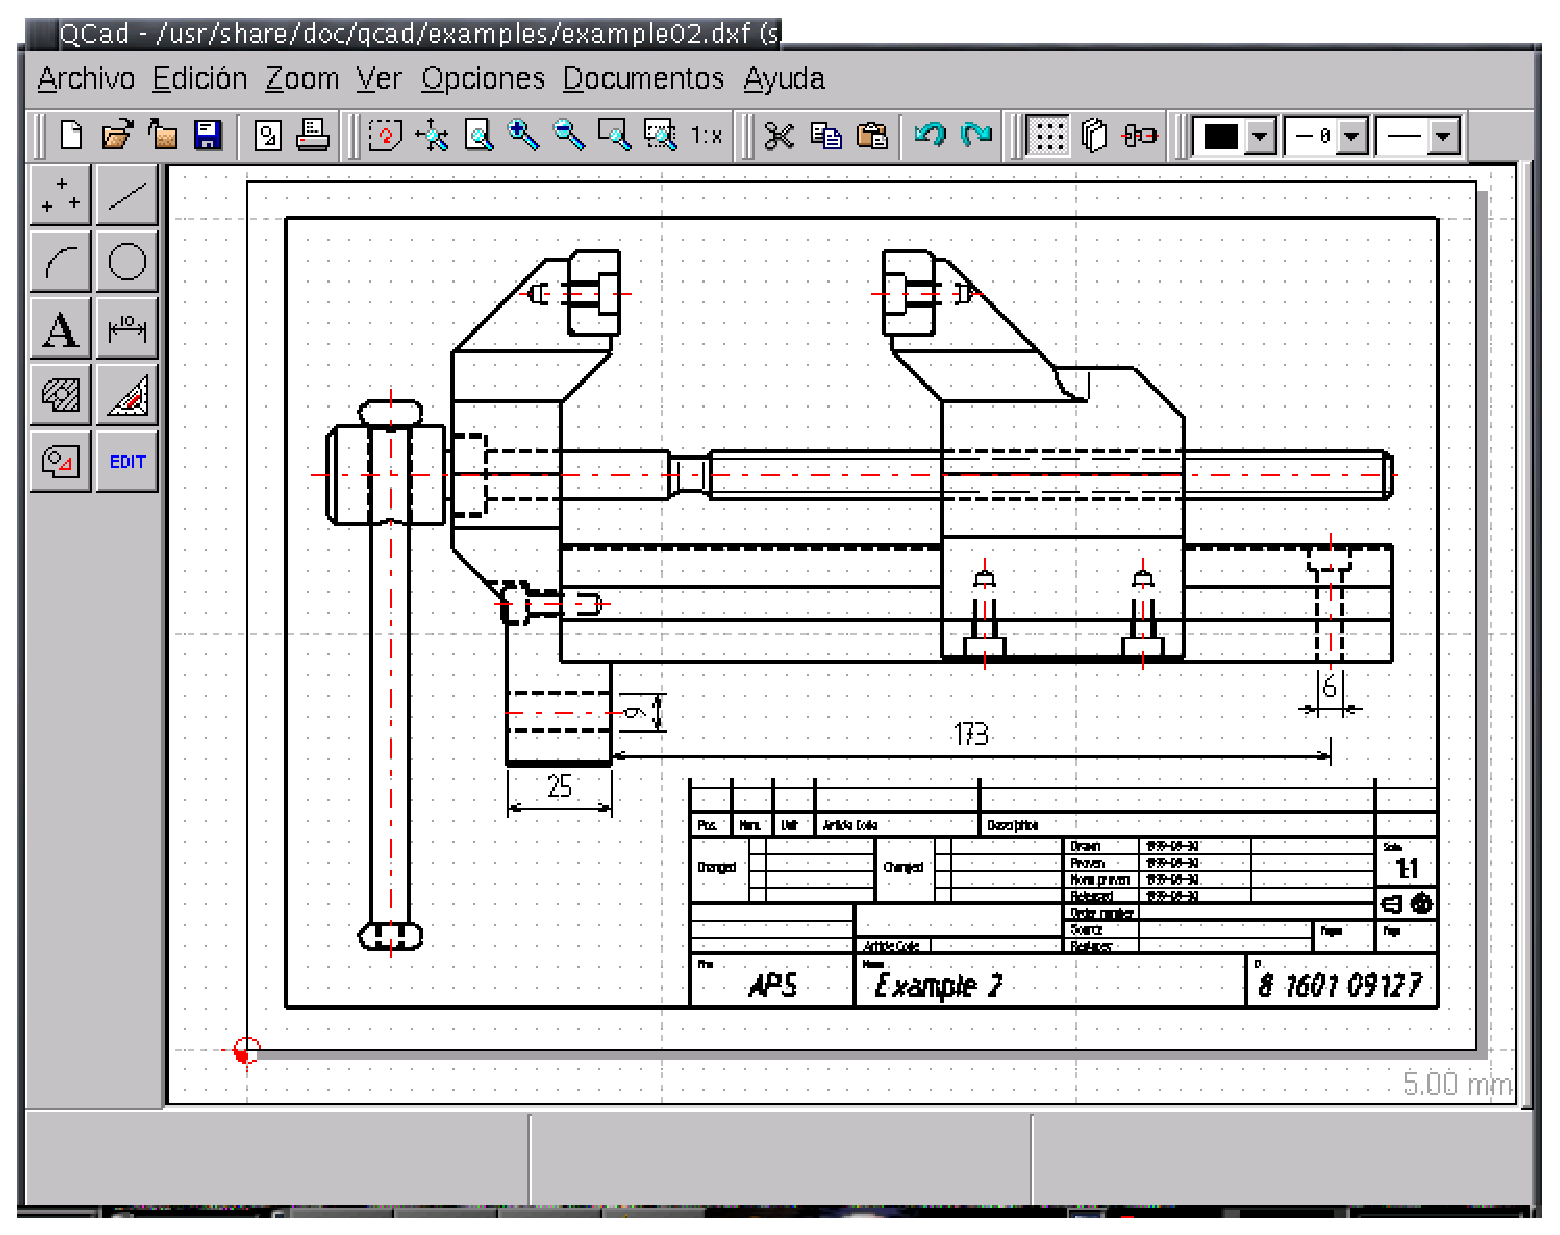
\includegraphics[width=0.88\textwidth]{imagenes/qcad_main.eps}
\caption{Ventana principal de QCad}
\end{figure}
